%%%%%%%%%%%%%%%%%%%%%%%%%%%%%%%%%%%%%%%%%%%%%%
\section{Beamline}
\label{sec:h4beamline}

The H4 beamline is extended to the NP04 cryostat in the newly constructed extension of EHN1. To produce particles in the momentum range of interest, 80 GeV/c pion beam from the the T2 primary target is impinged on a secondart Cu target to generate a tertiary beam. The tertiary particles are momentum and charged-selected and transported down the H4 beamline to the experimental area. The H4 beamline can operate in parallel with the H2 beamline minimize interference between the two ProtoDUNE experiments.

\subsection{H4 Beamline layout and optics}

A sketch of the H4 beamline layout is shown in Figure~\ref{fig:H4layout}. The first two dipole magnets (shown in red) after the secondary target are rotated by about 56$^\circ$ to move the beam downward towards the cryostat. The third dipole magnet (shown in green) is for sweeping the beam into one of the three beam windows.
\begin{cdrfigure}[H4 beamline layout]{H4layout}{Sketch of the H4 beamline layout in the region near the cryostat.}
  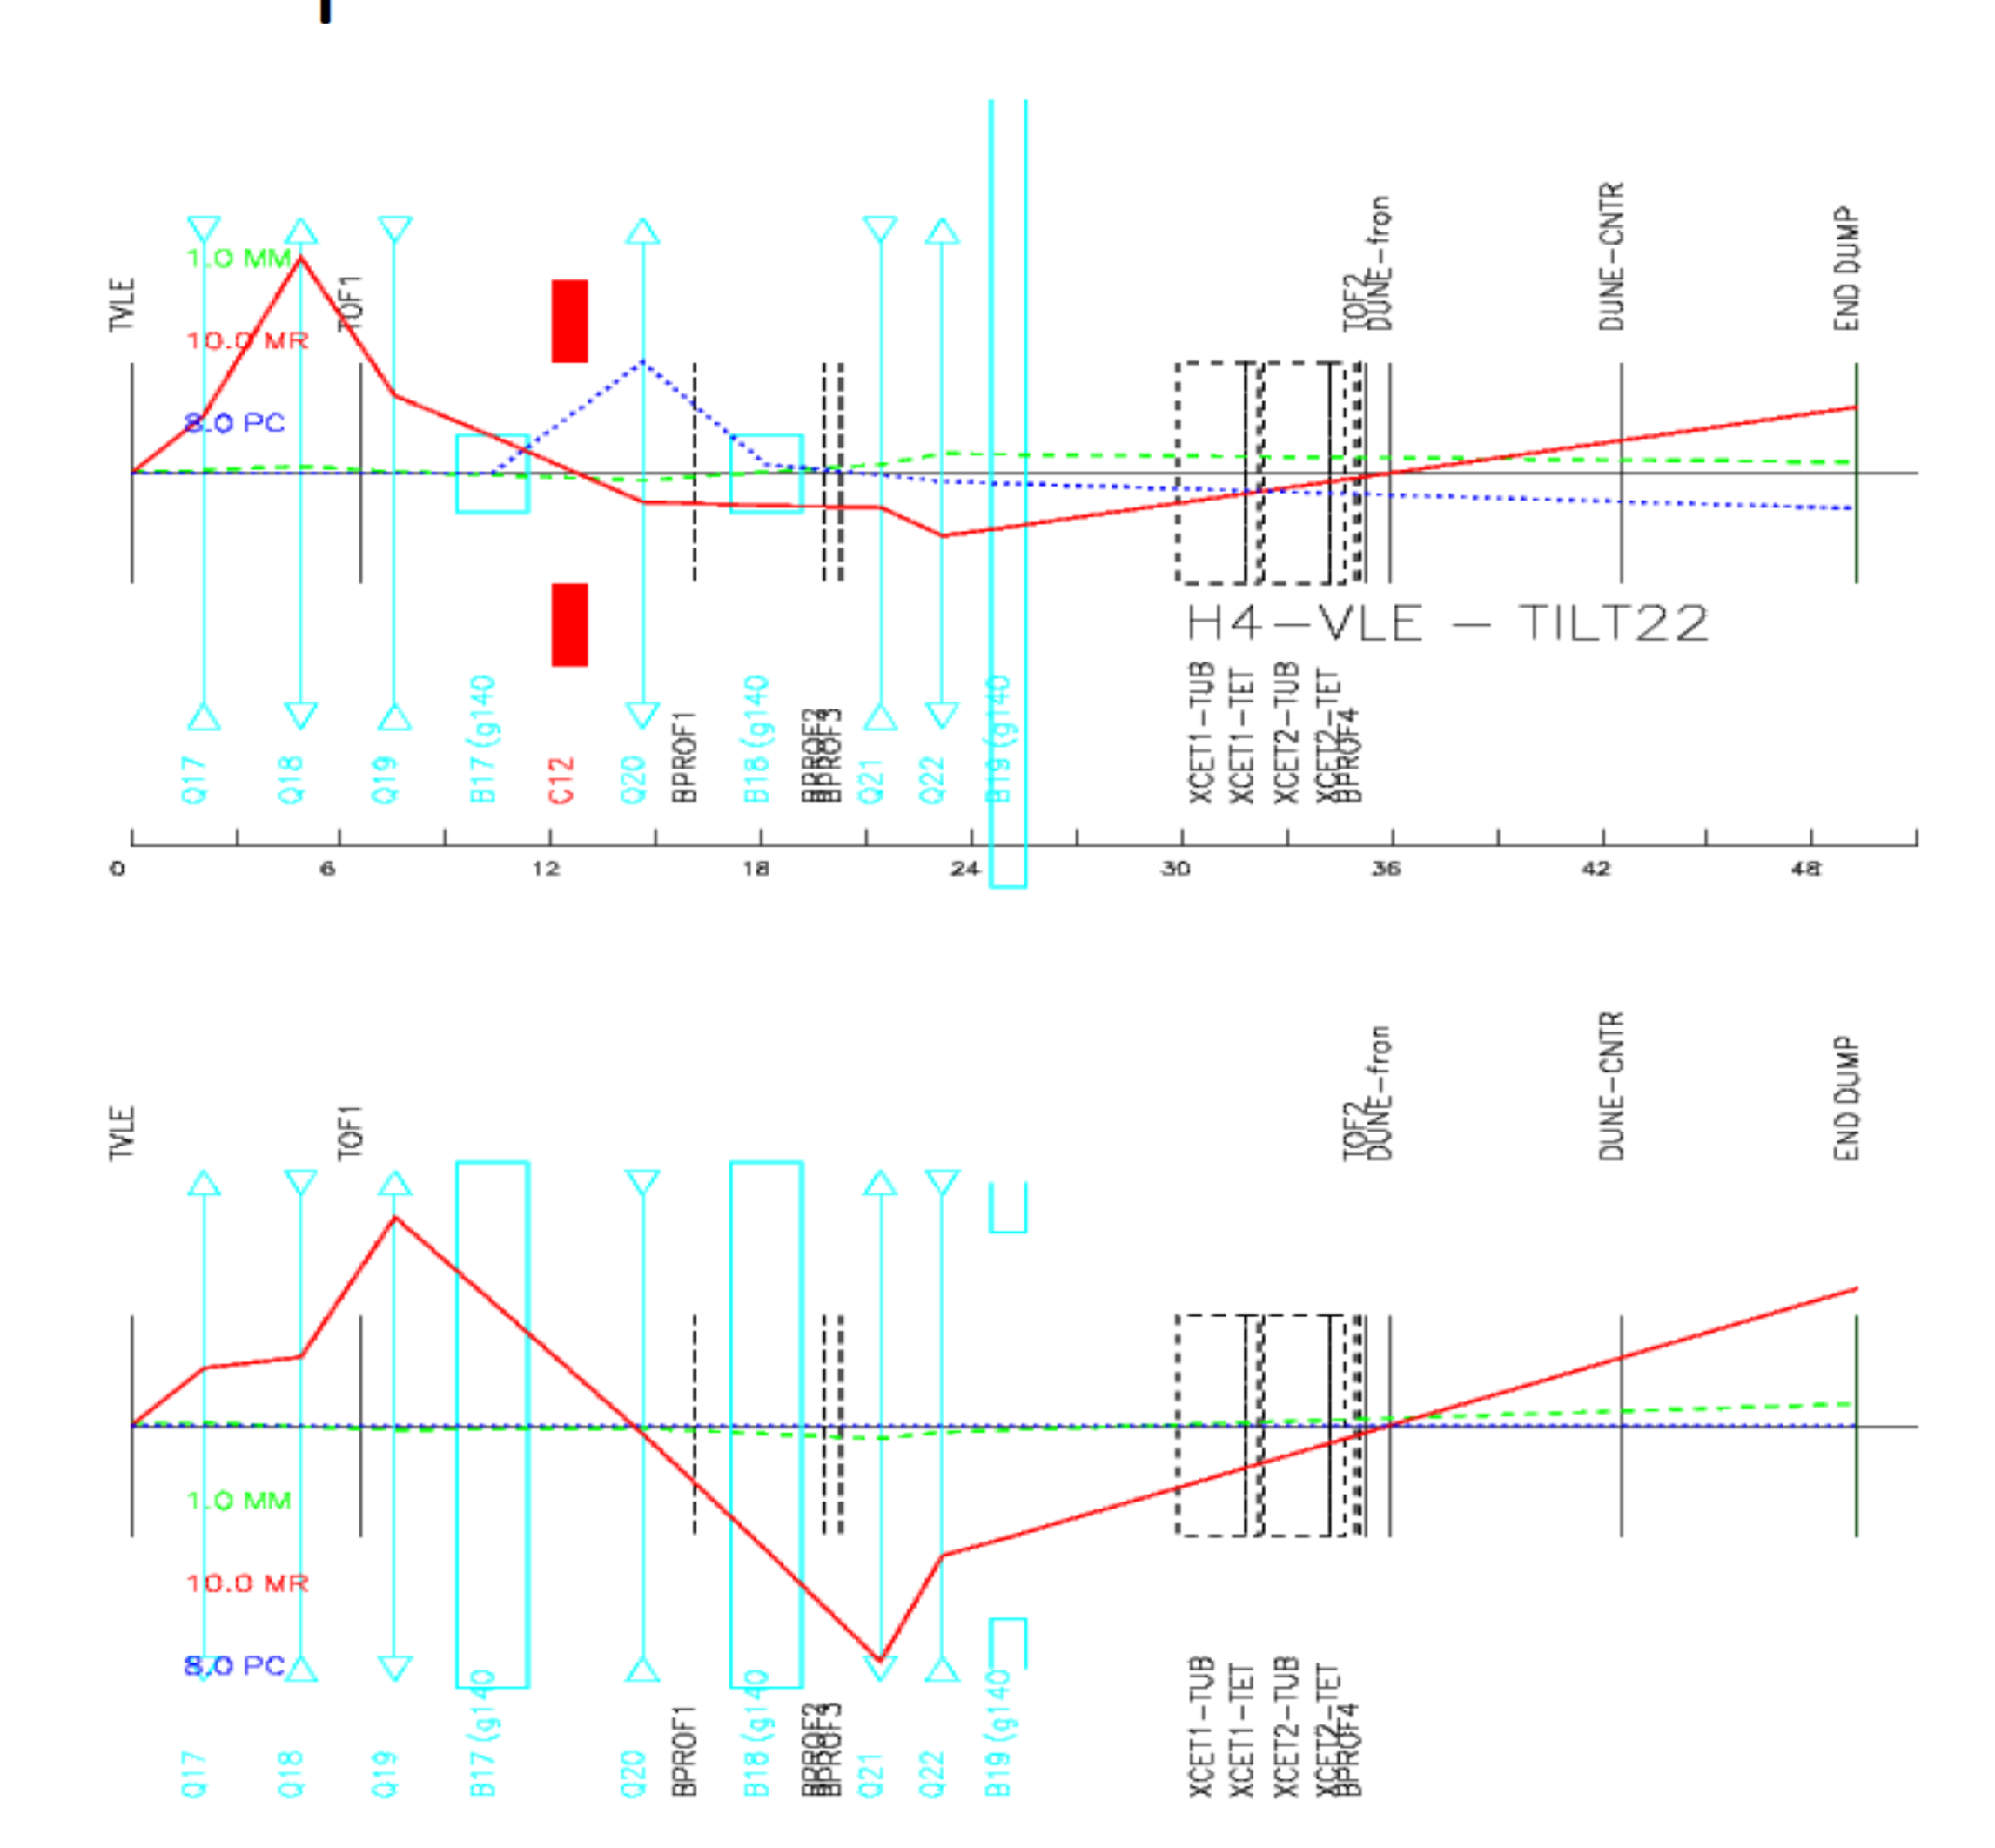
\includegraphics[width=0.95\textwidth]{beamline_H4layout.pdf}
\end{cdrfigure}


The beamline optics for the horizontal and vertical planes are shown in Figure~\ref{fig:beamoptics}. For this particular set of configuration, the beam is focused at the front of the cryostat. There are three sets of dipole magnet. The first two sets are for momentum selection and the last dipole (closest to the cryostat) is for sweeping the beam horizontally into one of the three beam windows.
\begin{cdrfigure}[H4 beam optics]{beamoptics}{H4 beamline optics for the horizontal (top) and vertical (bottom) planes. The secondary target is located on the left side of the plots and the front of the ProtoDUNE-SP cryostat is located at the beam focus point, at about 33m from the secondary target.}
  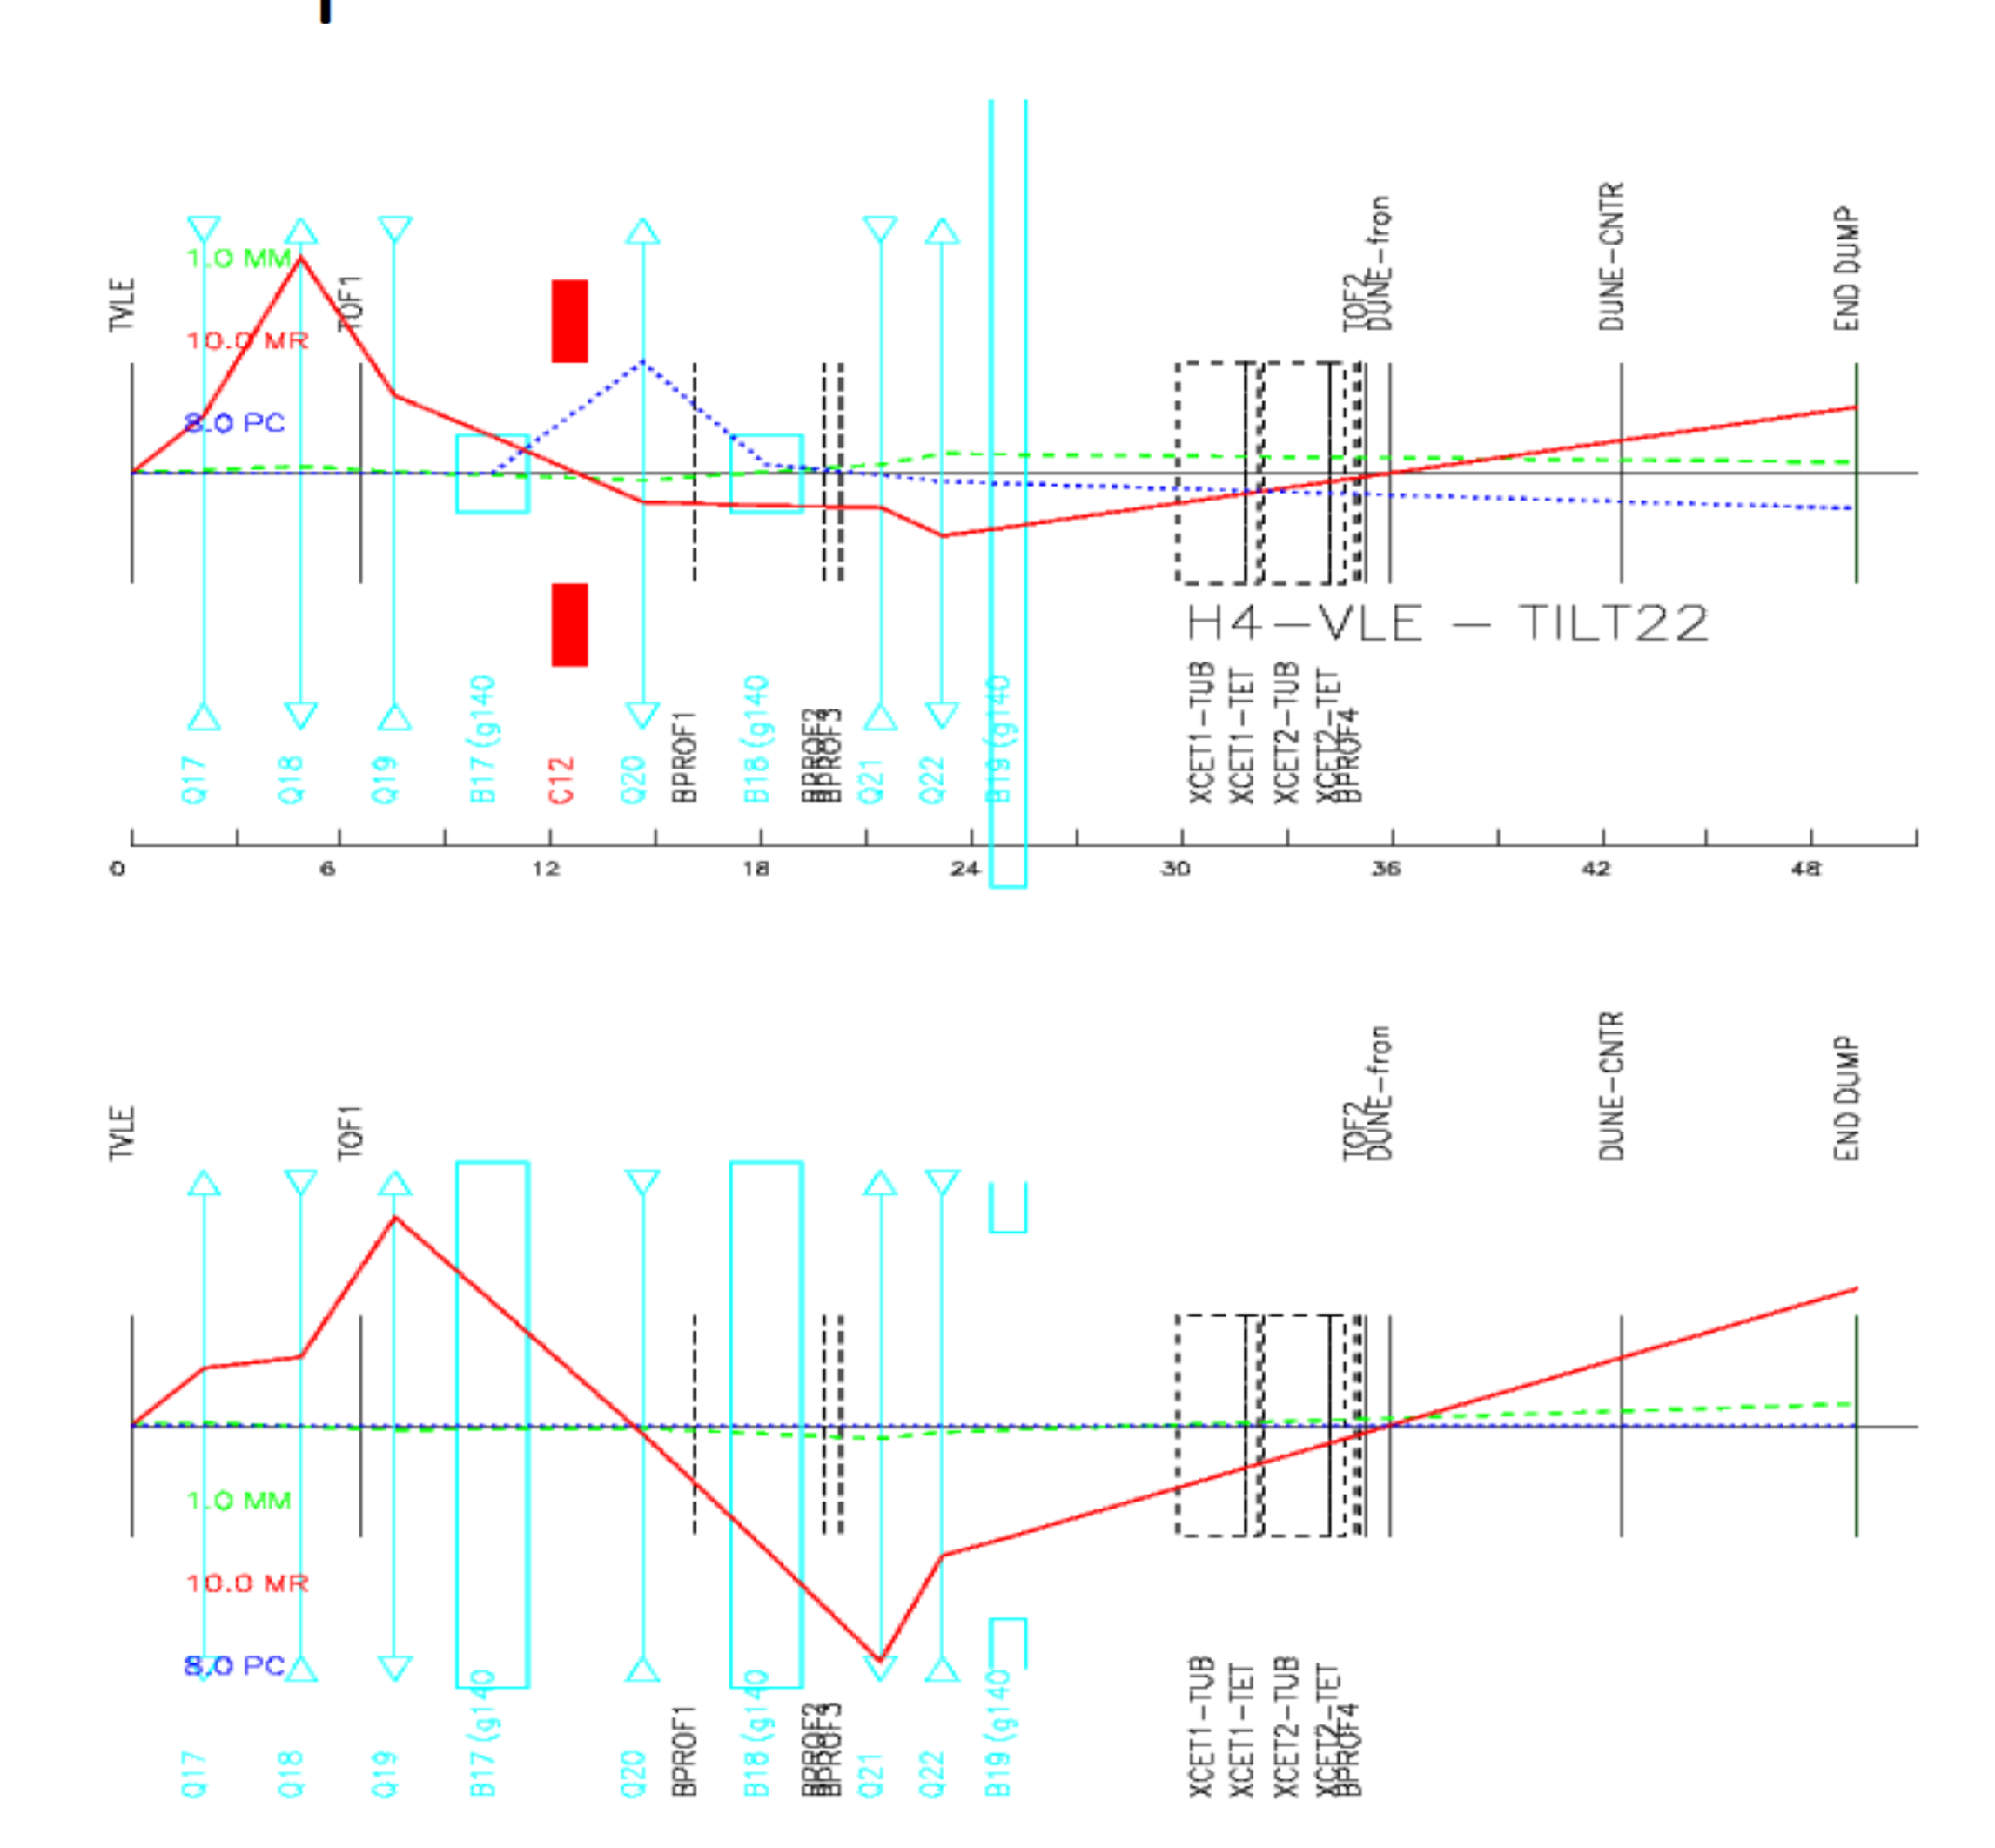
\includegraphics[width=0.95\textwidth]{beamline_H4Optics.pdf}
\end{cdrfigure}

\subsection{Beam properties}
\fixme{Need simulation results from Nikos}
\begin{itemize}
\item particle spectra
\item expected rates
\item expected beam dimensions 
\end{itemize}

\subsection{Muon halo}




